% Word count: 1123

\section{Design}
	\subsection{System Architecture Overview}
		The system will comprise of three main components:
		\begin{itemize}
			\item Management Server
			\item User Interface
			\item Disposable instances/containers
		\end{itemize}
		The system will also use existing ECS instances i.e  where backups are stored. Depending on the user of the system there may be multiple backup servers in different location (such as AWS regions) or for different data types (relational and non-relational databases).
		
		\begin{figure}[H]
			\setlength{\belowcaptionskip}{15pt plus 3pt minus 2pt}
			\caption{Diagram of System Architecture}
			\centering
			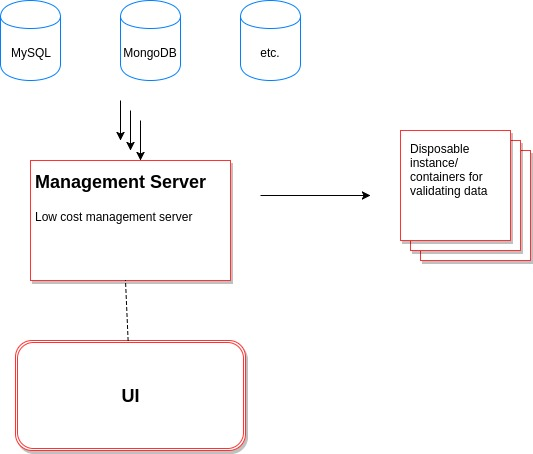
\includegraphics[scale=0.5,keepaspectratio]{diagram}
			\label{fig:diagram}
		\end{figure}
		
		\noindent \textbf{Management Server:} This will be a small low cost AWS instance on which the Jenkins automation server will be installed. The majority of the systems functionality will be carried out and/or orchestrated by this server. Jenkins jobs will copy the backups from their location to a disposable instance and implement the necessary steps to validate them such as importing and and reading.
		
		\noindent \textbf{User Interface:} This will provide a simple user interface (UI) for the system, implemented as a simple web app, hosted on AWS.It will allow users with little knowledge of Jenkins and AWS to perform backup restoration checks by adding a layer of abstraction. Users will be able to run restorations by providing the parameters such as the backup file and it's location. The UI will utilise the Jenkins API to run execute the restoration with the parameters provided.
		
		\noindent\textbf{Disposable Instances:} Disposable infrastructure will be used to perform the restoration. This will consist of EC2 instances running the necessary DBMS to perform the restoration. They can also be destroyed afterwards, destroying the data and therefore maintaining confidentiality.

	\subsection{Formal Modelling}
	\subsubsection{Sequence Diagrams}
		The main function of the systems have been demonstrated below in sequence diagrams. \autoref{fig:seq-run-restore} shows the process of running a single backup restore. This involves a user manually triggering a restoration using the web interface. This triggers a Jenkins job which automates the remaining steps:
		\begin{enumerate}
			\item Backup copied to \textit{restoration} server;
			\item Backup decrypted;
			\item Backup import into DBMS;
			\item Data read from DB;
		\end{enumerate}
		Upon completion the \textit{restoration} server is terminated.

		\autoref{fig:seq-schedule-restore} shows the process of a scheduling regular backup restoration tests. Again, this is triggered by a user from the web interface. The web interface will pass the JSON or XML configuration for a job to the Jenkins server. The server verify the backup server exists before creating the job.
		
		\autoref{fig:seq-delete-restore} Show the process of deleting an existing scheduled job. The user triggers this process from the web interface. This sends a delete commands to the Jenkins server via the API to remove the schedule job. The status of the command, indicating a successful or failed restore, is returned to the user.
		
		\begin{figure}[H]
			\setlength{\belowcaptionskip}{15pt plus 3pt minus 2pt}
			\caption{Run Restore}
			\centering
			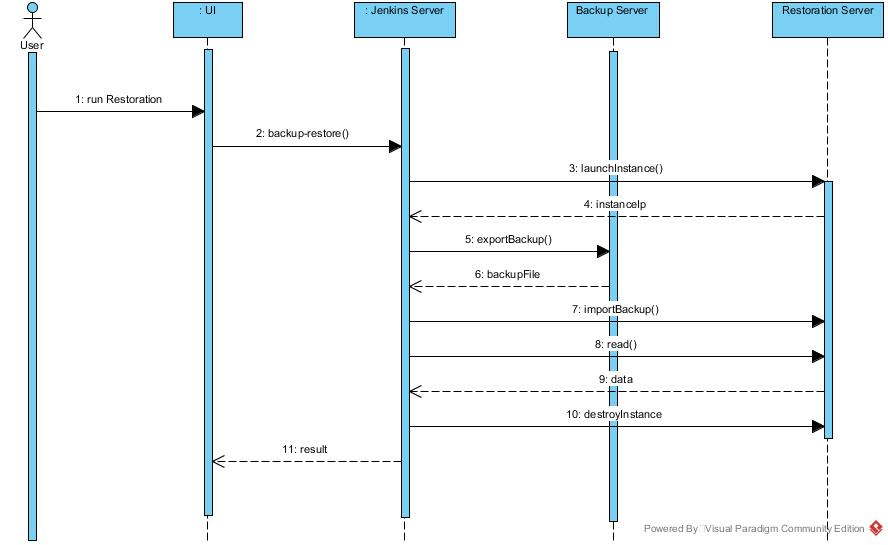
\includegraphics[width=\textwidth,keepaspectratio]{sequence-diagram-run-restore}
			\label{fig:seq-run-restore}
		\end{figure}
		
		\begin{figure}[H]
			\setlength{\belowcaptionskip}{15pt plus 3pt minus 2pt}
			\caption{Schedule Regular Restore}
			\centering
			%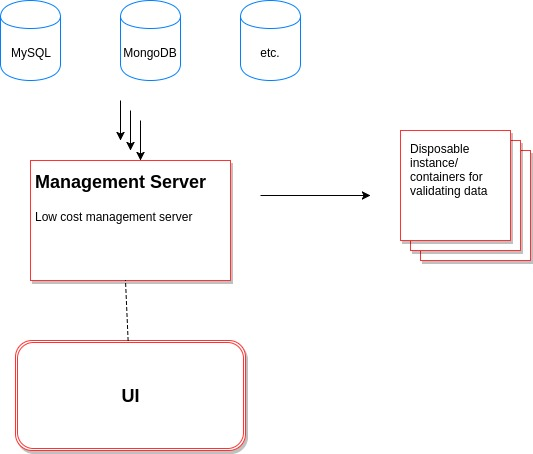
\includegraphics[width=\textwidth,height=\textheight,keepaspectratio]{diagram}
			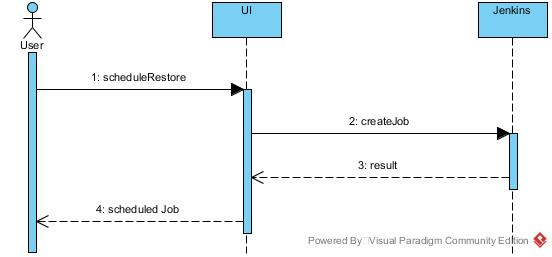
\includegraphics[width=\textwidth,keepaspectratio]{sequence-diagram-schedule-restore}
			\label{fig:seq-schedule-restore}
		\end{figure}
		
		\begin{figure}[H]
			\setlength{\belowcaptionskip}{15pt plus 3pt minus 2pt}
			\caption{Delete Scheduled Restore}
			\centering
			%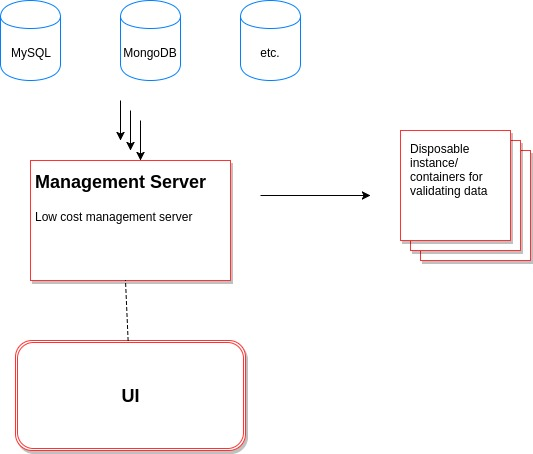
\includegraphics[width=\textwidth,height=\textheight,keepaspectratio]{diagram}
			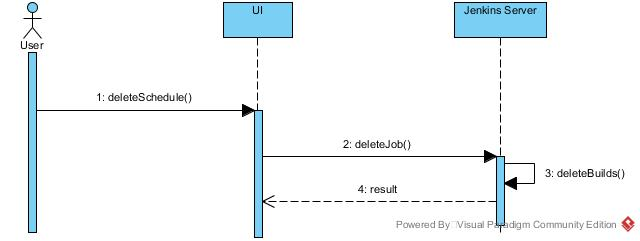
\includegraphics[width=\textwidth,keepaspectratio]{sequence-diagram-delete-schedule}
			\label{fig:seq-delete-restore}
		\end{figure}
	
	\subsubsection{User Stories} \label{user-stories}
    
    \note[id=RB]{The expanded user stories in Table 1 look good. The table appears to overlap the page number.}
    
		User stories are provided in \autoref{table:user-stories}. Two types of system users and their privileges are described below;
		
		\textbf{Managers} control security aspects of the system:
		\begin{itemize}
			\item Add and remove regular users;
			\item Manage SSH keys and decryption keys.
		\end{itemize}
		\textbf{Regular Users} will perform the day-to-day tasks of the system:
		\begin{itemize}
			\item Perform resorations;
			\item Schedule restorations;
			\item View restoration results;
		\end{itemize}
		
		\begin{table}[H]
			\centering
			\setlength{\belowcaptionskip}{15pt plus 3pt minus 2pt}
			\caption{User Stories}
                         
			\begin{tabular}{|l|p{0.1\linewidth}|p{0.35\linewidth}|p{0.35\linewidth}|} \hline
				\textbf{\#} & \textbf{As a} & \textbf{I want to be able to} & \textbf{so that} \\ \hline
				US1 & manager & implement a user system & I control who can run backup restores \\ \hline
				US1.1 & manager & add my team members to the system & they can run backup restores \\ \hline
				US1.2 & manager & remove users from the system & former team members no longer have access \\ \hline
				US2 & manager & add and control sensitive information within the system & I can implement a security policy \\ \hline
				US2.2 & manager & securely store credentials within the system & they don't need to be entered every time a restore is executed \\ \hline
				US2.3 & manager & add SSH keys for backup server & the system has secure access backup server \\ \hline
				US2.4 & manager & add decryption keys for backups & encrypted backups can be decrypted for testing \\ \hline
				US2.5 & manager & delete SSH keys & expired/outdated credentials are no longer stored \\ \hline
				US2.6 & manager & delete decryption keys & expired/outdated credentials are no longer stored \\ \hline
				US3 & manager & execute all same tasks as a regular user & I don't need a second set of credentials to run restores myself \\ \hline
				US4 & user & login & I can run restores \\ \hline
				US5 & user & logout & I avoid potential unauthorised access \\ \hline
				US6 & user & run a test restoration of a backup & I can verify that the backup exists, is a valid file, and is readable \\ \hline
				US6.1 & user & run a test by filling out a simple form with basic parameters (location, filename) of the backup to test & I can easily run a restore of a specific backup without needing to worry about the implementation \\ \hline
				US6.2 & user & view the current status \added[id=RB]{of} a running restoration & I can review the progress of long running restores \\ \hline
				US6.3 & user & check if a backup failed or succeeded & I can immediately investigate any failed backups \\ \hline
				US7 & user & create a schedule of automated restores for a given backup & I don't have to manually execute them myself on a regular basis \\ \hline
				US7.1 & user & choose the frequency of automated restores within a schedule, from daily through weekly to monthly & I control how often different backups are tested \\ \hline
				US7.2 & user & check if an automated restoration has started & I can verify my schedule is working correctly \\ \hline
				US7.3 & user & check the results of an automated restore & I can immediately investigate any failed backups \\ \hline
				US7.4 & user & view the all past results of an automated restore schedule & view the consistency of my backups success \\ \hline
				US7.5 & user & modify a scheduled restore & I can change the frequency of a scheduled restore \\ \hline
				US7.6 & user & the parameters of a schedule & any changes to the backups, such as location, will be reflect in the restoration schedule \\ \hline
				US7.7 & user & delete regularly scheduled restores & old backups/deleted backups are no longer tested \\ \hline 

US8 & user & view feedback of a failed restore & I might gain an insight into the fault in the backup \\ \hline
				US9 & user & notified when a restoration fails & silent, unnoticed fails are avoided \\ \hline
			\end{tabular}
			\label{table:user-stories}
		\end{table}
		

        
	\subsection{Front End Design}
	\subsubsection{Wireframes}
	
		Wireframes for the frontend are shown below. 
        
        \autoref{fig:homepage} shows the homepage. It includes the following components:
		\begin{itemize}
			\item Form for running a restore;
			\item Form for creating a restore schedule;
			\item List of schedules (including links).
		\end{itemize}
		\autoref{fig:scheduled} shows the details and past results of a scheduled restore.
		
		
		\begin{figure}[H]
			\setlength{\belowcaptionskip}{15pt plus 3pt minus 2pt}
			\caption{Homepage}
			\centering
			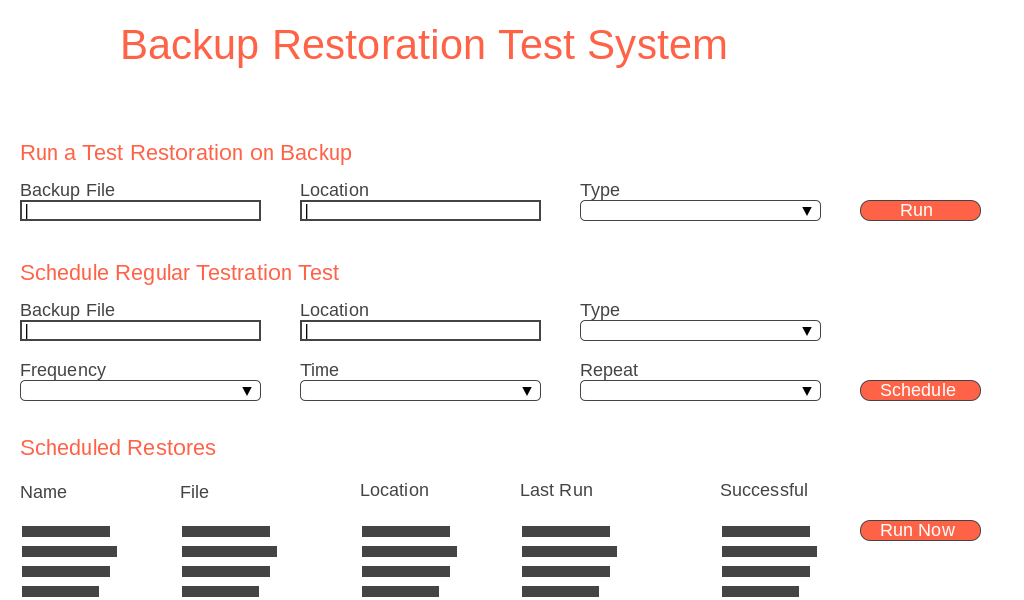
\includegraphics[width=\textwidth,keepaspectratio]{wireframe-homepage}
			\label{fig:homepage}
		\end{figure}
		
		\begin{figure}[H]
			\setlength{\belowcaptionskip}{15pt plus 3pt minus 2pt}
			\caption{Scheduled Restore}
			\centering
			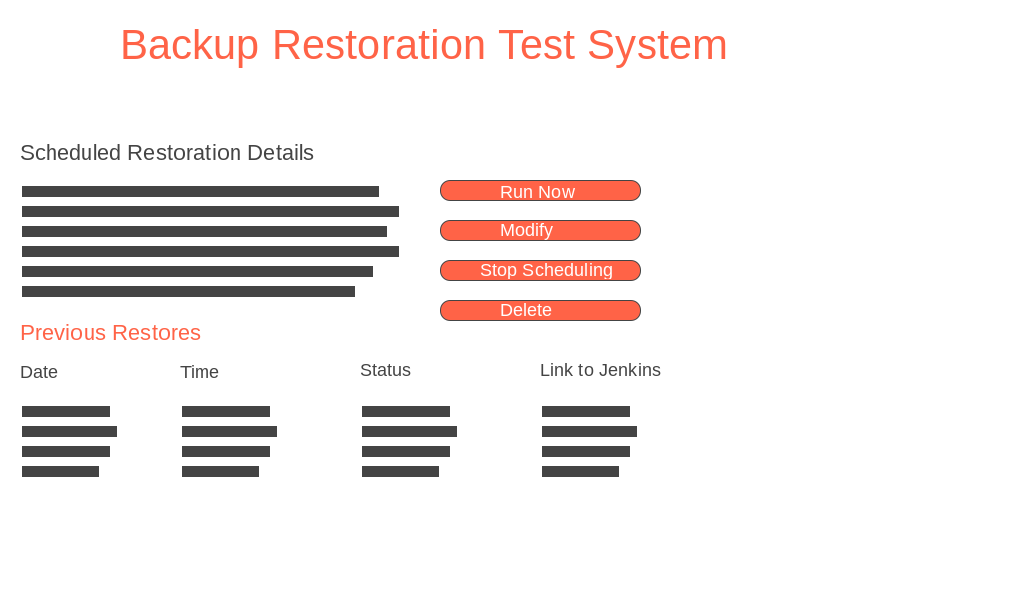
\includegraphics[width=\textwidth,keepaspectratio]{wireframe-scheduled-restore}
			\label{fig:scheduled}
		\end{figure}
	